\documentclass[a4paper, 10pt]{article}
\usepackage{fullpage} % changes the margin
\usepackage[english]{babel}
\usepackage[utf8]{inputenc}
\usepackage{hyperref}
\usepackage{xcolor}
\usepackage{graphicx}
\usepackage{array}
\usepackage{float}
\usepackage{longtable}
\usepackage[bottom]{footmisc}
\usepackage{cite}
\usepackage{parskip}
\usepackage{subcaption}
\usepackage{amssymb}
\usepackage{amsmath}
\usepackage{listings}
\usepackage[nocenter]{qtree}
\usepackage{tree-dvips}

\hypersetup{
	colorlinks=true,       % false: boxed links; true: colored links
	linkcolor=blue,        % color of internal links
	citecolor=blue,        % color of links to bibliography
	filecolor=magenta,     % color of file links
	urlcolor=blue
}

%\setlength{\parindent}{0cm}
\newcommand{\code}[1]{\texttt{#1}}
\newcommand{\suchthat}[0]{\hspace{1mm}|\hspace{1mm}}
\renewcommand{\arraystretch}{1.4}
\definecolor{statement}{gray}{0.5}

\graphicspath{{img/}}

\begin{document}

\noindent
\begin{flushright}
    \large\textbf{Miguel Alcón Doganoc} \\
    Algorithms for VLSI \\
    \today
\end{flushright}

\noindent
{\huge{\textbf{Exercises on physical design}}}

\section{Quadratic placement}
{\color{statement} 
Show the two linear system of equations for the x and y coordinates.
}

Our system of equations is
\[
     AX - b_x = 0\text{, and } AY - b_y = 0
\]
where
\[
    A = \begin{bmatrix}
        3 & 0 & -1 & -1 \\
        0 & 5 & -1 & 1 \\
        -1 & -1 & 4 & 0 \\
        -1 & -1 & 0 & 4
    \end{bmatrix}\hspace{3mm}
    X = \begin{bmatrix}
        X_a \\
        X_b \\
        X_c \\
        X_d \\
    \end{bmatrix}\hspace{3mm}
    b_x = \begin{bmatrix}
        5 & 6 & 5 & 10
    \end{bmatrix}\hspace{3mm}
    Y = \begin{bmatrix}
        Y_a \\
        Y_b \\
        Y_c \\
        Y_d
    \end{bmatrix}  \hspace{3mm}
    b_y = \begin{bmatrix}
        0 & 12 & 2 & 5
    \end{bmatrix}
\]
So, the final systems are
\[
    \begin{cases}
        3 X_a - X_c - X_d - 5 = 0  \\
        5 X_b - X_c - X_d - 6 = 0 \\
        - X_a - X_b + 4 X_c - 5 = 0 \\
        - X_a - X_b + 4X_d - 10 = 0 \\
    \end{cases}\hspace{3mm}
    \begin{cases}
        3 Y_a - Y_c - Y_d = 0  \\
        5 Y_b - Y_c - Y_d - 12 = 0 \\
        - Y_a - Y_b + 4 Y_c - 2 = 0 \\
        - Y_a - Y_b + 4Y_d - 5 = 0 \\
    \end{cases}
\]
{\color{statement} 
Solve the systems of equations and draw the final solution in a 2D plot.
}

The final solution is
\[
    a = (\frac{177}{44},\frac{59}{44})\hspace{8mm}b = (\frac{115}{44},\frac{141}{44})\hspace{8mm}c = (\frac{32}{11},\frac{18}{11})\hspace{8mm}d = (\frac{183}{41},\frac{105}{44})    
\]

\begin{figure}[htbp]
    \centering
    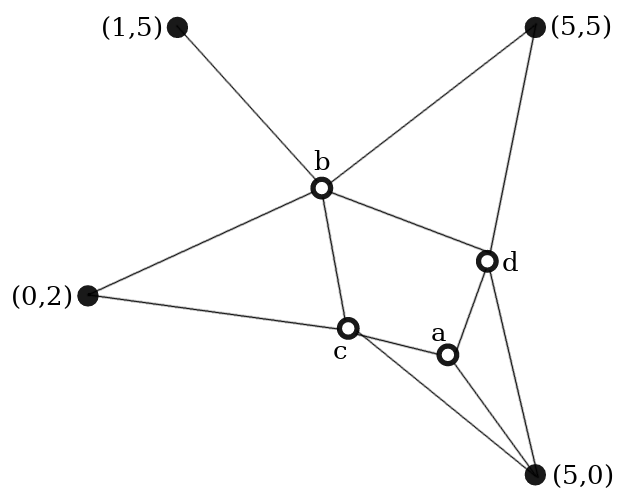
\includegraphics[width=0.5\linewidth]{1_qplacement.png}
\end{figure}
\newpage
\section{Channel Routing}
{\color{statement} Draw the vertical constraint graph without splitting the nets.}
\begin{figure}[htbp]
    \centering
    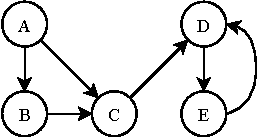
\includegraphics[width=0.3\linewidth]{2_vcg.pdf}
\end{figure}


{\color{statement} Determine the zone representation for the nets.}

\begin{figure}[htbp]
    \centering
    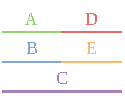
\includegraphics[width=0.2\linewidth]{2_zr.pdf}
\end{figure}

{\color{statement} Draw the vertical constraint graph with net splitting.}

\begin{figure}[htbp]
    \centering
    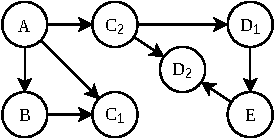
\includegraphics[width=0.3\linewidth]{2_vcg_split.pdf}
\end{figure}


{\color{statement} Find the minimum number of required tracks with net splitting and without net splitting.}

Since without net splitting nodes $D$ and $E$ creates a loop in the VCG, it is impossible to route this channel.  With net splitting, I found the number of tracks after applying the Dogleg Left-Edge algorithm, which is 5. 

{\color{statement} Use the Dogleg Left-Edge algorithm to route this channel. For each track, state which nets are assigned. Draw the final routed channel.}

The assignment of nets to tracks is specified at the right of the route diagram.
\begin{figure}[H]
    \centering
    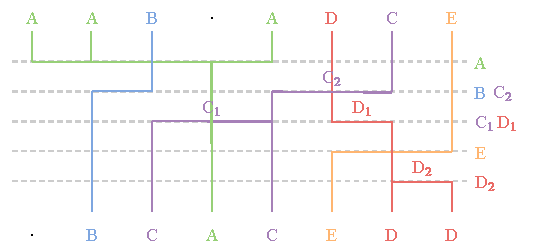
\includegraphics[width=0.9\linewidth]{2_route.pdf}
\end{figure}
\newpage
\section{Sequence pairs}
\Tree [.V [.H c a ] [.H e [.H b d ] ] ]

\end{document}